\documentclass{article}
\usepackage{spconf,amsmath,amssymb,amsthm,graphicx,booktabs,hyperref}
\hypersetup{hidelinks}

% Conservative float/display spacing tuning; official margins and 9pt size are unchanged.
\setlength{\floatsep}{2pt plus 1pt minus 1pt}
\setlength{\textfloatsep}{2pt plus 1pt minus 1pt}
\setlength{\intextsep}{2pt plus 1pt minus 1pt}
\setlength{\abovedisplayskip}{2pt plus 1pt minus 1pt}
\setlength{\belowdisplayskip}{2pt plus 1pt minus 1pt}
\setlength{\abovecaptionskip}{2pt plus 1pt minus 1pt}
\setlength{\belowcaptionskip}{1pt}

% Light bibliography spacing tuning only: the inter-entry gap and list top
% separation are minimized so the reference-only page can carry more verified
% references. The official 9pt reference font (spconf \ninept) and all
% margins are unchanged.
\makeatletter
\def\thebibliography#1{\section{References}\list
 {[\arabic{enumi}]}{\settowidth\labelwidth{[#1]}\leftmargin\labelwidth
 \advance\leftmargin\labelsep
 \itemsep\z@ \topsep 2\p@
 \usecounter{enumi}}
 \def\newblock{\hskip .11em plus .33em minus .07em}
 \sloppy\clubpenalty4000\widowpenalty4000
 \sfcode`\.=1000\relax}
\makeatother

\newtheorem{definition}{Definition}
\newtheorem{assumption}{Assumption}
\newtheorem{lemma}{Lemma}
\newtheorem{theorem}{Theorem}
\newtheorem{proposition}{Proposition}
\newtheorem{corollary}{Corollary}
\newcommand{\E}{\mathbb{E}}
\newcommand{\R}{\mathbb{R}}
\newcommand{\D}{\Delta}
\newcommand{\G}{\mathcal G}

% Compact author block: drop the blank row after the name row and tighten the
% title area (official fonts/margins unchanged; needed for the 4-page limit).
\makeatletter
\def\name#1{\gdef\@name{{\em #1}}}
\def\@maketitle{\newpage
 \null
 \vskip 1em \begin{center}
 {\large \bf \@title \par} \vskip .75em {\large \lineskip .5em
\begin{tabular}[t]{c}\@name \\ \@address
 \end{tabular}\par} \end{center}
 \par
 \vskip 1em}
\makeatother

\title{RC-ZOQO: CERTIFYING RESOLUTION LIMITS IN QUANTIZED ZEROTH-ORDER OPTIMIZATION}
\name{Dongxu Liu$^{1,\ast}$\thanks{$\ast$Corresponding author.}, Wenjia Shi$^{2}$, Dongyang Liu$^{3}$, Xiang Luo$^{4}$}
\address{$^{1}$School of Artificial Intelligence, Jilin University, Changchun, China\\
$^{2}$College of Computer Science and Technology, Jilin University, Changchun, China\\
$^{3}$Yingcai Honors College, University of Electronic Science and Technology of China, Chengdu, China\\
$^{4}$College of Software, Jilin University, Changchun, China\\
{\footnotesize E-mail: liudx9924@mails.jlu.edu.cn, shiwj2126@mails.jlu.edu.cn, 2024310102018@std.uestc.edu.cn, luoxiang5525@mails.jlu.edu.cn}}

\begin{document}
\ninept
\maketitle
\vspace{-0.75em}

\begin{abstract}
Quantized zeroth-order (ZO) optimizers keep optimizing on a discrete grid, but once the nominal probe
or update falls below one grid step the run enters a \emph{one-grid regime}: queries keep flowing while
the grid cannot express the intended motion. We identify
and characterize this terminal resolution wall: for quadratics, exact phase-averaged floor laws show
the RMS stationarity floor is linear in the grid spacing and curvature-weighted, so each extra bit
approximately halves it. RC-ZOQO then audits, from function values alone, whether a $\gamma$-sufficient
decrease remains observable, with an exact finite-sample certificate: the false-stop probability is
$(1-p_{\gamma,m}(x))^K$, and $K$ failures certify $p_{\gamma,m}(x)\le1-\delta^{1/K}$ at confidence
$1-\delta$. On INT4/INT8 MNIST MLPs the audit stops a resolution-exhausted full model
($89.3$\%/$33.8$\% fewer post-floor/total queries, no accuracy loss) and continues a head-only block,
recovering $+1.14$ points a schedule stop discards.
Code is available at \url{https://github.com/ldx825/RC-ZOQO_ICASSP-2027}.
\end{abstract}

\begin{keywords}
zeroth-order optimization, quantization, low-bit training, black-box optimization, resolution certificate
\end{keywords}

\section{Introduction}
Quantized zeroth-order (ZO) adaptation makes forward-only fine-tuning possible at deployment precision: ZOQO keeps parameters, perturbations, and updates quantized \cite{bar2025zoqo}; QuZO uses stochastic rounding for low-bit large-model fine-tuning \cite{zhou2025quzo}; QZO perturbs quantization scales \cite{shang2026qzo}; CAQ-ZO aligns the query geometry with the companding quantizer \cite{shu2026caq}; and forward-only fine-tuning is now routine \cite{malladi2023mezo}, building on two-point ZO estimation \cite{kiefer1952,spall1992spsa,nesterov2017random,duchi2015optimal,liu2020primer}, ZO-signSGD \cite{liu2019zosign}, sparse-gradient ZO \cite{cai2022zoro}, and evolution strategies \cite{salimans2017es}. These methods answer how to keep optimizing on a discrete grid; we ask \emph{when the grid itself has become the bottleneck}. Once the nominal probe or update falls below one grid step, the loop can only round the intended motion away or force a one-grid update, while every iteration still costs queries. Forced one-grid updates can oscillate near a grid-misaligned optimum even under an exact sign oracle, and endpoint clipping can reverse a comparison; in our INT4 MLP run, post-entry forced updates spend $299$ extra queries and drift $0.26$ points.

A fixed schedule is a poor proxy: crossing the threshold is neither necessary nor sufficient for resolution exhaustion---it discards recoverable progress when the floor is not yet reached and keeps spending queries when it is. We exhibit both failure modes in one protocol: an exhausted full model, and a head-only block that crosses the same threshold while one-grid decreases remain valuable (Section~\ref{sec:gate} recovers $+1.14$ points by auditing instead of stopping on schedule). One-grid entry should trigger a state check, not a stop.

We first price the grid, then turn the terminal regime into a black-box statistical decision. For quadratics, exact floor laws (Theorem~\ref{thm:floor}) give the representable stationarity floor in closed form, $F_{\D}=\D\|H\|_F/\sqrt{12}$, with each extra bit approximately halving it. RC-ZOQO then \emph{audits} the state (Definition~\ref{def:audit}): it tests up to $K$ one-grid Rademacher directions at a fixed state and stops when none satisfies \eqref{eq:audit}. No gradient, Hessian, or Lipschitz constant is needed---an exact chord decomposition (Lemma~\ref{lem:chord}) uses only queried values---and the guarantee is a finite-sample statement about the audit distribution: if $p_{\gamma,m}(x)$ is the probability that a sampled direction is $\gamma$-useful, the false-stop probability is exactly $(1-p_{\gamma,m}(x))^K$, and $K$ failures certify $p_{\gamma,m}(x)\le1-\delta^{1/K}$ at confidence $1-\delta$ (Theorem~\ref{thm:cert}); accepted steps form a finite sequence (Proposition~\ref{prop:fin}).

Our contributions are threefold. (i) \textbf{Resolution wall characterization}: exact curvature-weighted floor laws, the bit law, spectral bounds for general curvature, and a range--resolution relation (Appendix). (ii) \textbf{A state-based black-box certificate}: the audit, its exact chord decomposition, the finite-sample certificate, the finite accepted-step bound, and resolution invariance. (iii) \textbf{Stop/continue validation}: on INT4/INT8 MNIST MLPs the audit stops an exhausted full model ($89.3$\%/$33.8$\% fewer post-floor/total like-for-like queries, no accuracy loss) and continues a head-only block, recovering $+1.14$ points a schedule stop discards.

RC-ZOQO is a diagnostic certificate for existing quantized ZO loops, not a replacement optimizer (cf.\ \cite{bergou2020stp}); it does not remove the floor, it detects when a fixed-resolution run has reached it. Query budgets matter when every evaluation is paid for \cite{chen2017zoo,ilyas2018limited}; sufficient-decrease polling is classical in direct search \cite{gratton2015pds} and quantization error is classical \cite{hou2019quantized}; ours is the quantized one-grid terminal regime.

\section{Background and Problem Setup}
\label{sec:background}
\subsection{Quantized ZO updates}
Following the fully quantized setting of ZOQO \cite{bar2025zoqo}, a uniform $b$-bit quantizer covers a range of width $D$ with grid spacing $\D_b=D/(2^b-1)$. Nominal probe/update scales are quantized to multiples of $\D_b$; ZOQO enforces one grid step once a nominal scale drops below the spacing, giving two queries and the clamped sign update $x^{\pm}_{\mathrm{p}}=\operatorname{clamp}(x\pm ar)$, $c=\operatorname{sign}[f(x^{+}_{\mathrm{p}})-f(x^{-}_{\mathrm{p}})]$, $x_{\mathrm{next}}\leftarrow\operatorname{clamp}(x-\alpha cr)$, with quantized probe/update magnitudes $a,\alpha$. Low-bit formats and quantized gradients are standard \cite{dettmers2022int8,frantar2023gptq,lin2024awq,courbariaux2016binarized,hubara2017qnn,gupta2015deep,jacob2018quantization,micikevicius2018mixed,alistarh2017qsgd} (survey: \cite{krishnamoorthi2018whitepaper}).

\begin{definition}[One-grid regime]
A quantized ZO run is in the \emph{one-grid regime} when its nominal probe or update would fall below one grid spacing and the realized nonzero scale is one grid step ($a=\D_b$ and/or $\alpha=\D_b$). Crossing this threshold triggers auditing; it is not by itself a stopping criterion.
\end{definition}

\subsection{Notation and assumptions}
Let $x\in\R^d$ and let $\G_{\D}$ denote the scalar lattice of spacing $\D$ applied coordinate-wise, with $x^\star$ a continuous minimizer.
\begin{assumption}[Random grid phase]
\label{ass:phase}
For phase-averaged floor calculations, the phase of $x^\star$ relative to each scalar cell is i.i.d. uniform in $[-\D/2,\D/2]$.
\end{assumption}

\begin{assumption}[Local smoothness and admissible queries]
\label{ass:smooth}
For the audit analysis, $f$ is $L$-smooth on every queried segment, and audit directions are restricted to coordinates with sufficient margin so that $x\pm ar$ and the one-grid update do not clip, isolating resolution effects from clipping; RC-ZOQO uses an active set of non-clipping coordinates.
\end{assumption}

\section{Resolution Limits of Quantized ZO}
\label{sec:floor}
\subsection{Phase-averaged floor}
For a quadratic objective $f(x)=\frac12(x-x^\star)^\top H(x-x^\star)$ with $H\succeq0$, the phase-averaged nearest-grid error $e=\bar x-x^\star$ satisfies $\E[e]=0$ and $\E[ee^\top]=\frac{\D^2}{12}I$ (Lemma~\ref{lem:phase}, Appendix).

\begin{theorem}[Curvature-weighted nearest-grid law]
\label{thm:floor}
Under Assumption~\ref{ass:phase},
\begin{align}
\E[f(\bar x)-f^\star] &= \frac{\D^2}{24}\operatorname{tr}(H), \label{eq:objfloor}\\
\E\|\nabla f(\bar x)\|_2^2 &= \frac{\D^2}{12}\operatorname{tr}(H^2). \label{eq:gradfloor}
\end{align}
Hence the RMS nearest-grid stationarity scale is $F_{\D}=\frac{\D}{\sqrt{12}}\|H\|_F$. For diagonal $H$, nearest scalar quantization minimizes $f$ over the grid, making \eqref{eq:objfloor}--\eqref{eq:gradfloor} exact grid-constrained floors.
\end{theorem}

For non-axis-aligned curvature, Corollary~\ref{cor:gridfloor} (Appendix) bounds the discrete optimum.

Combining Theorem~\ref{thm:floor} with $\D_b=D/(2^b-1)$ yields the bit law $F_b=D\|H\|_F/(\sqrt{12}(2^b-1))$, i.e., $b\ge\lceil\log_2(1+D\|H\|_F/(\sqrt{12}\epsilon))\rceil$ for target RMS stationarity scale $\epsilon$. It is exact for axis-aligned quadratics, and $F_{b+1}/F_b\to1/2$: each extra bit approximately halves the stationarity scale and quarters the objective scale.

Two examples show why the floor matters: for $f(x)=\frac12(x-\D/2)^2$, an exact-sign one-grid update from $x_0=0$ alternates $0\leftrightarrow\D$, so the best cell is reached yet forced updates continue; and for $f=x_1+0.75x_2$ on range $[0,3a]$ at $x=(0,1.5a)$, $r=(1,-1)$, the true derivative $0.25>0$ but the clamped comparison gives $-0.5a<0$. RC-ZOQO avoids clipped chords and tests whether one-grid motion remains resolvable.

\section{Resolution-Certified ZOQO}
\label{sec:method}
\subsection{Resolution audit}
RC-ZOQO activates when the base quantized ZO optimizer reaches the one-grid regime; an audit direction then samples $m\le q$ coordinates uniformly without replacement from the admissible (non-clipping) set $\mathcal A\subseteq[d]$ ($q:=|\mathcal A|$), with independent Rademacher signs ($r\in\{-1,0,1\}^d$, $\|r\|_0=m$), probed symmetrically at magnitude $a$.

\begin{definition}[Resolution audit]
\label{def:audit}
For forcing constant $\gamma\ge0$, an audit direction is declared successful if
\begin{equation}
\min_{\sigma\in\{-1,+1\}} f(x+\sigma ar)
\le f(x)-\gamma a^2m.
\label{eq:audit}
\end{equation}
\end{definition}
A successful direction is executed immediately: the better of $x\pm ar$ becomes the next iterate, so a successful audit both certifies and performs a one-grid decrease, reusing the queried point. RC-ZOQO tests up to $K$ independent directions with \eqref{eq:audit}; if all $K$ fail, the run stops---a certificate on the sampled directions, not a proof that no progress exists. $\gamma$ sets the minimum one-grid decrease deemed worth further queries, not whether any descent exists.

The forcing constant sets the gate's strictness: $\gamma=0$ certifies any strict decrease (on a noisy floor the audit never stops), larger $\gamma$ stops earlier; the experiments report $\gamma\in\{0,0.05,0.25\}$. A self-calibrated $\gamma^\star$ from the one-grid two-point history ($[0.40,0.62]$ INT4, $[1.36,1.85]$ INT8) is a conservative heuristic, not an oracle for remaining progress.

The audit minimum over two one-grid moves has a closed form in the queried function values.

\begin{lemma}[Exact chord decomposition]
\label{lem:chord}
For any direction $r$ with $\|r\|_0=m$, define the one-grid slope and curvature statistics $\widehat s_r(x)=\frac{f(x+ar)-f(x-ar)}{2a}$ and $\widehat c_r(x)=\frac{f(x+ar)+f(x-ar)-2f(x)}{2a^2}$. Then
\begin{align}
f(x\pm ar)-f(x)&=a^2\widehat c_r(x)\pm a\,\widehat s_r(x),\nonumber\\
\min_{\sigma\in\{-1,+1\}} f(x+\sigma ar)-f(x)&=a^2\widehat c_r(x)-a\,|\widehat s_r(x)|,
\label{eq:chordmin}
\end{align}
so \eqref{eq:audit} is equivalent to $|\widehat s_r(x)|-a\,\widehat c_r(x)\ge\gamma am$.
\end{lemma}

This test is the entire audit: $\widehat s_r$ is the observable chord slope and $\widehat c_r$ the curvature penalty paid on it, both computed from the two queried endpoints and the cached $f(x)$. No gradient, Hessian, global smoothness constant, or ambient dimension $d$ enters the decision---only the $m$ probed coordinates---which is why the audit remains executable at neural scale.

\subsection{A finite-sample resolution certificate}
What does a run learn from $K$ failed audits? Define the sampled useful-direction mass $p_{\gamma,m}(x)=\Pr_r[A_r(x)=1]$, where $A_r(x)=\mathbf 1\{\min_{\sigma}f(x+\sigma ar)\le f(x)-\gamma a^2m\}$ and $r$ is drawn from the audit distribution---a quantity defined purely by what the audit observes. The next result gives an exact finite-sample interpretation of $K$ failed audits.

\begin{theorem}[Finite-sample resolution certificate]
\label{thm:cert}
Fix $x$, $\gamma\ge0$, $m$, and the audit distribution; assume failed audits leave $x$ unchanged and directions are independent. Then the probability of observing $K$ consecutive failures is exactly $(1-p_{\gamma,m}(x))^K$; consequently, if $p_{\gamma,m}(x)\ge\varepsilon$ for some $\varepsilon\in(0,1)$, the probability that RC-ZOQO stops after $K$ failed audits is at most $(1-\varepsilon)^K$. Conversely, after observing $K$ failures and no success, for any $\delta\in(0,1)$ the one-sided bound $p_{\gamma,m}(x)\le1-\delta^{1/K}$ holds with confidence at least $1-\delta$.
\end{theorem}

Both parts are exact, with no smoothness or moment assumption; the theorem certifies scarcity of useful directions under the audit distribution, not the nonexistence of a descent direction. With $K{=}15$, $\delta{=}0.05$ this reads $p_{\gamma,m}(x)\le1-0.05^{1/15}\approx18.1\%$; if $p_{\gamma,m}(x)\ge0.2$, the false-stop probability is at most $0.8^{15}\approx3.52\%$. Each audit costs at most $2K+1$ evaluations per state: the cached $f(x)$ plus two probes per direction. A gradient-norm-only lower bound cannot generally remain dimension-free for sparse random audits, because a concentrated gradient may be missed by the sampled support; the Appendix records the classical condition and why it becomes vacuous at neural scale.

\begin{proposition}[Finite audited-phase termination]
\label{prop:fin}
Suppose $\gamma>0$ and $f\ge f_{\inf}$ on all queried states. Every accepted audit satisfies \eqref{eq:audit}, so $N_{\mathrm{acc}}\le\lfloor(f(x_0)-f_{\inf})/(\gamma a^2m)\rfloor$; after the last accepted step every audit fails, so RC-ZOQO stops within $K$ audits with the certificate of Theorem~\ref{thm:cert}. We deliberately do not claim convergence to a continuous stationary point: at fixed resolution the audited phase ends in a certified stop.
\end{proposition}


The audit decision is a property of the state geometry, not the bit width: INT4 and INT8 runs can behave alike at matched normalized states.
\begin{corollary}[Resolution invariance for quadratics]
\label{cor:invariant}
Let $f(x)=\frac12(x-x^\star)^\top H(x-x^\star)$, write $x=x^\star+\D z$, and use a one-grid audit $a=\D$. Then \eqref{eq:audit} is equivalent to $|z^\top Hr|\ge\frac12r^\top Hr+\gamma m$, which is independent of $\D$; if a ZO-sign step also moves exactly one grid step without clipping, then $z^+=z-\operatorname{sign}(z^\top Hr)r$, so the normalized dynamics are resolution-invariant.
\end{corollary}

Inside the representable cell, no one-grid move strictly decreases a diagonal quadratic when $\gamma=0$ (Appendix): the audit falls silent instead of forcing oscillatory moves.

\section{Experiments}
\label{sec:exp}
For Theorem~\ref{thm:floor} we use $d\in\{16,64,256\}$, five resolutions, 5000 random phases, three Hessian spectra: relative errors of \eqref{eq:objfloor}/\eqref{eq:gradfloor} are $1.09\%$/$1.85\%$, and log--log RMS-floor slopes versus $\D$ are $0.99994$--$1.00041$ (Fig.~\ref{fig:floor}).

\begin{figure}[t]
\centering
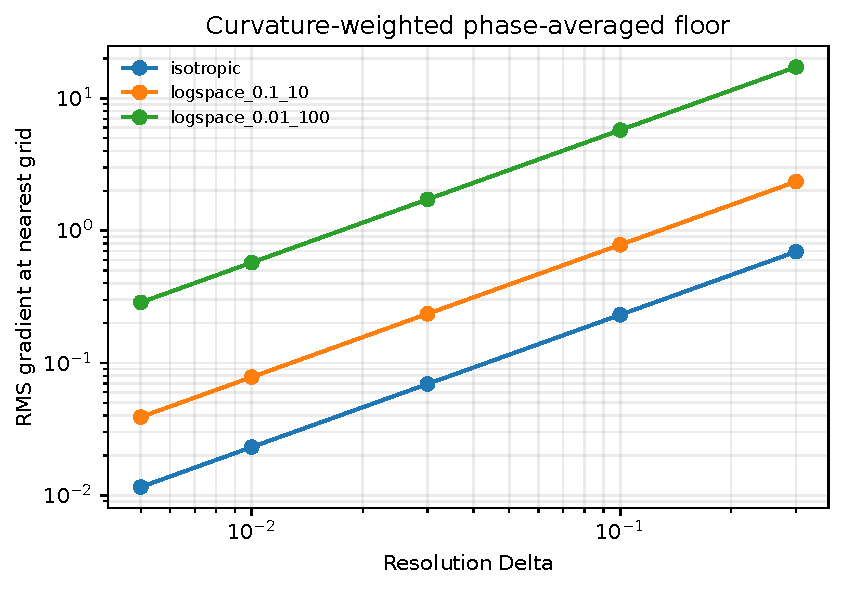
\includegraphics[width=0.70\columnwidth]{figures/fig11_curvature_weighted_floor.pdf}
\caption{RMS stationarity floor vs.\ grid spacing: unit log--log slope; curvature changes the coefficient.}
\label{fig:floor}
\end{figure}

Theorem~\ref{thm:cert} is exact, so validation targets its inputs: the mass $p_{\gamma,m}(x)$ and the false-stop law $(1-p_{\gamma,m}(x))^K$. Across 90 $(q,k,m)$ configurations ($q$: coordinates, $k$: nonzero gradient entries, $m$: support size) at fixed quadratic states ($10^5$ draws each), empirical success frequencies reproduce the $m/q$ support-hit scaling and the predicted phase transition, respecting the appendix's gradient-based bound (no $3\sigma$ violation).

\subsection{Stopping at a resolution floor}
We use a 784--256--128--10 MLP on MNIST: the full-precision checkpoint reaches $96.72$\% and direct INT4 quantization $96.32$\% (INT8 essentially lossless). The black-box objective is cross-entropy on a fixed 4096-example subset (grid spacings $\D_4=0.0439$, $\D_8=0.0026$); all runs use 400 iterations, three seeds, and one-grid entry at iteration 251, where RC-ZOQO audits with $\gamma=0.05$, $m=1024$, and $K=15$.

Pre-entry RC-ZOQO matches the clipping-safe baseline; fixed ZOQO then keeps forcing one-grid moves, drifting from $96.22$\% to $95.96$\% over 299 queries. RC-ZOQO rejects the first floor audit in all three seeds and stops: 32 post-floor queries instead of 299 ($89.3$\% fewer) and $33.8$\% fewer total queries than the trajectory-matched clipping-safe baseline (523 vs.~790), avoiding the $0.26$-point drift. All three seeds observe $K=15$ consecutive failures, certifying at $95\%$ confidence that fewer than $18.1\%$ of sampled directions remain $\gamma$-useful. At $\gamma=0$ it accepts one strict decrease, stalls, and ends at $95.22$\%: pure descent at a noisy floor is not accuracy-preserving. At INT8 the audit likewise spends 32 post-floor queries instead of 299 at comparable accuracy ($96.83$\% vs.~$96.81$\%), supporting the resolution-invariant interpretation.

\begin{table}[t]
\centering
\small
\renewcommand{\arraystretch}{0.92}
\setlength{\tabcolsep}{2.6pt}
\caption{MNIST MLP quantized-ZO adaptation (3 seeds): full model (top), head-only gate (bottom); ``Post'' $=$ queries after one-grid entry.}
\label{tab:real}
\begin{tabular}{lrrrr}
\toprule
Method & Bits & Acc. (\%) $\uparrow$ & Queries $\downarrow$ & Post $\downarrow$\\
\midrule
ZOQO & 4 & 95.96 & 802 & 299\\
Clip-safe ZOQO & 4 & 96.02 & 790 & 299\\
\textbf{RC-ZOQO} & \textbf{4} & \textbf{96.22} & \textbf{523} & \textbf{32}\\
ZOQO & 8 & 96.81 & 802 & 299\\
\textbf{RC-ZOQO} & \textbf{8} & \textbf{96.83} & \textbf{535} & \textbf{32}\\
\bottomrule
\end{tabular}

\vspace{1pt}
\begin{tabular}{lrrr}
\toprule
Head-only policy & Acc. (\%) $\uparrow$ & Queries $\downarrow$ & Accepted\\
\midrule
Stop at entry & 93.85 & 118 & 0\\
Audit $\gamma=\gamma^\star$, $m=16$ & 93.85 & 149 & 0.0\\
Audit $\gamma=0.25$, $m=16$ & 94.26 & 178 & 2.7\\
Audit $\gamma=0.05$, $m=16$ & 94.99 & 256 & 21.7\\
Forced updates (no audit) & 94.93 & 398 & {--}\\
Audit $\gamma=0$, $m=64$ & \textbf{96.08} & 663 & 103.7\\
\bottomrule
\end{tabular}
\end{table}

\subsection{Continuing despite schedule entry}
\label{sec:gate}
To exercise the accepting side we repeat the protocol on the $1{,}290$-parameter classifier head of the same MLP (one-grid entry at iteration $60$, all audits at $K=15$): INT4 quantization leaves the block at $96.68$\%, and the shared pre-floor trajectory ends at $93.85$\% when the one-grid regime begins, so the floor is not yet reached. The same $\gamma=0.05$ rule that stopped the full model here continues: $21.7$ accepted steps reach $94.99$\% at $256$ queries, $+1.14$ points over the schedule stop ($93.85$\% at $118$). Table~\ref{tab:real} traces the frontier: forced updates reach $94.93$\% at $398$ queries, $\gamma=0$ steps to $96.08$\% at $663$, while $\gamma=0.25$ stops after $2.7$ accepted steps and $\gamma^\star$ stops at entry; at INT8 the gate stops after one accepted step ($96.75$\% vs.~$96.72$\%). ``Accepted'' counts executed steps; the $96.08$\% of $\gamma=0$ is a looser policy than $\gamma=0.05$. The audit is a state-based gate whose strictness sets the continue/stop frontier---not a schedule rule---and accepted steps pay their own cost. A $13\times$ larger LoRA-style block (16,640 parameters, rank 16 \cite{hu2022lora}) reproduces the stopping side ($\gamma\ge0.05$ stops at entry; $\gamma=0$ never stops). The two cases are the two sides of the same decision problem: one-grid entry triggers auditing, whereas the current state decides between stop and continue.

\noindent\textbf{Scope and limitations.} RC-ZOQO diagnoses when a fixed-resolution run has reached the floor of Theorem~\ref{thm:floor}; a failed audit certifies the absence of sampled $\gamma$-sufficient one-grid directions, not local optimality; the certificate needs no smoothness constant.

\enlargethispage{4\baselineskip}
\section{Conclusion}
Schedules cannot tell when a quantized ZO run stops carrying signal:
once the nominal motion falls below one step, queries keep flowing
while updates cannot move the model---the terminal resolution wall.
We price the wall (curvature-weighted floor laws; each bit roughly
halves the floor) and turn it into a testable state: a resolution
audit over function values with an exact finite-sample certificate
and a finite accepted-descent bound. On INT4/INT8 MNIST MLPs it stops
an exhausted full model ($89.3$\%/$33.8$\% fewer post-floor/total
queries, no accuracy loss) and continues a head-only block, recovering
$+1.14$ points a schedule stop discards.

\section{Appendix: Proofs}
\subsection{Proofs of Lemma~\ref{lem:phase} and Theorem~\ref{thm:floor}}
\begin{lemma}[Random-phase moments]
\label{lem:phase}
Let $\bar x$ be the nearest-grid quantization of $x^\star$ and $e=\bar x-x^\star$. Under Assumption~\ref{ass:phase}, $\E[e]=0$ and $\E[ee^\top]=\frac{\D^2}{12}I$.
\end{lemma}
\emph{Proof of Lemma~\ref{lem:phase}.} For each coordinate, $e_j=\bar x_j-x_j^\star$ is uniform on $[-\D/2,\D/2]$ by Assumption~\ref{ass:phase}, so $\E[e_j]=0$, $\E[e_j^2]=\D^2/12$, and $\E[e_je_k]=0$ for $j\ne k$; hence $\E[e]=0$ and $\E[ee^\top]=(\D^2/12)I$.

\emph{Proof of Theorem~\ref{thm:floor}.} Since $e^\top He=\operatorname{tr}(Hee^\top)$, $f(\bar x)-f^\star=\frac12\operatorname{tr}(Hee^\top)$; substituting Lemma~\ref{lem:phase} in expectation,
\[
\E[f(\bar x)-f^\star]=\tfrac12\operatorname{tr}\big(H\,\E[ee^\top]\big)=\tfrac12\operatorname{tr}\big(H\,\tfrac{\D^2}{12}I\big)=\tfrac{\D^2}{24}\operatorname{tr}(H),
\]
which is \eqref{eq:objfloor}. Similarly $\nabla f(\bar x)=He$ gives $\E\|\nabla f(\bar x)\|_2^2=\operatorname{tr}(H^2\E[ee^\top])=\frac{\D^2}{12}\operatorname{tr}(H^2)$, i.e., \eqref{eq:gradfloor}, and $F_{\D}=(\D/\sqrt{12})\|H\|_F$; for diagonal $H$ each coordinate minimizes independently at the nearest grid point of $x_j^\star$, making \eqref{eq:objfloor}--\eqref{eq:gradfloor} exact.

\subsection{Proof of Corollary~\ref{cor:gridfloor} and auxiliary facts}
\begin{corollary}[General quadratic grid-floor bounds]
\label{cor:gridfloor}
Under Assumption~\ref{ass:phase}, for $H\succ0$ with lattice minimizer $x_{\D}^\star$, writing $\lambda_{-}\le\lambda_{+}$ for the extreme eigenvalues of $H$: $\E[f(x_{\D}^\star)-f^\star]\in\frac{d\D^2}{24}[\lambda_{-},\lambda_{+}]$ and $\E\|\nabla f(x_{\D}^\star)\|_2^2\in\frac{d\D^2}{12}[\lambda_{-}^2,\lambda_{+}^2]$.
\end{corollary}
\emph{Proof of Corollary~\ref{cor:gridfloor}.} Let $\bar x$ be the coordinate-wise nearest lattice point of $x^\star$, so $\delta_{\D}=\|\bar x-x^\star\|$ and $\E[\delta_{\D}^2]=d\D^2/12$ (Lemma~\ref{lem:phase}). \emph{Objective:} since $x_{\D}^\star$ minimizes $f$ on the lattice, $f(x_{\D}^\star)-f^\star\le\frac12\lambda_+\delta_{\D}^2$; conversely, strong convexity and the lattice membership of $x_{\D}^\star$ give $f(x_{\D}^\star)-f^\star\ge\frac12\lambda_-\delta_{\D}^2$, giving the interval. \emph{Gradient:} $\|\nabla f(x_{\D}^\star)\|_2^2=(x_{\D}^\star-x^\star)^\top H^2(x_{\D}^\star-x^\star)\ge\lambda_-^2\delta_{\D}^2$; and $H^2\preceq\lambda_+H$ (eigenvalues $\lambda_i^2\le\lambda_+\lambda_i$) bounds the same quantity by $2\lambda_+[f(x_{\D}^\star)-f^\star]\le\lambda_+^2\delta_{\D}^2$; substituting $\E[\delta_{\D}^2]$ completes the interval.

\emph{Auxiliary facts.} (a)~A uniform $b$-bit quantizer over width $D$ has step $\rho=D/(2^b-1)$ and span $(2^b-1)\rho$, so covering span $W$ with margin $h$ per side needs $W+2h\le(2^b-1)\rho$. (b)~For diagonal $H\succeq0$, $|z^\top Hr|\le\sum_j|z_j|h_j|r_j|\le\frac12r^\top Hr$ when $|z_j|<\frac12$ on the support, and \eqref{eq:chordmin} at $\gamma=0$ then keeps the audit minimum above $f(x)$: the audit falls silent inside the cell.

\subsection{Proofs of Lemma~\ref{lem:chord}, Thm.~\ref{thm:cert}, Prop.~\ref{prop:fin}, and Cor.~\ref{cor:invariant}}
\emph{Proof of Lemma~\ref{lem:chord}.} The definitions give $\frac12[f(x+ar)-f(x-ar)]=a\widehat s_r$ and $\frac12[f(x+ar)+f(x-ar)-2f(x)]=a^2\widehat c_r$; adding them gives $f(x+ar)-f(x)=a\widehat s_r+a^2\widehat c_r$, subtracting gives $f(x-ar)-f(x)=-a\widehat s_r+a^2\widehat c_r$, and minimizing over the sign gives $a^2\widehat c_r-a|\widehat s_r|$, so comparing with $-\gamma a^2m$ yields the test.

\emph{Proof of Theorem~\ref{thm:cert}.} Failed audits leave $x$ unchanged, so with $p=p_{\gamma,m}(x)$ and independence, $\Pr[\text{$K$ failures}]=(1-p)^K$; if $p\ge\varepsilon$ this is at most $(1-\varepsilon)^K$, bounding false stops. Conversely, if $p>1-\delta^{1/K}$ then $\Pr[\text{$K$ failures}]<\delta$; hence $p\le1-\delta^{1/K}$ holds at confidence $1-\delta$ (exact one-sided Clopper--Pearson).

\emph{Proof of Proposition~\ref{prop:fin}.} Each accepted audit decreases $f$ by at least $\gamma a^2m>0$; telescoping gives $f(x_0)-f(x_{N_{\mathrm{acc}}})\ge N_{\mathrm{acc}}\gamma a^2m$, and $f\ge f_{\inf}$ caps $N_{\mathrm{acc}}\le\lfloor(f(x_0)-f_{\inf})/(\gamma a^2m)\rfloor$. Each audit consumes one unit of the cap or fails; after $K$ failures the run stops certified by Theorem~\ref{thm:cert}.

\emph{Proof of Corollary~\ref{cor:invariant}.} Substituting $x=x^\star+\D z$, $a=\D$ gives $(z+\sigma r)^\top H(z+\sigma r)-z^\top Hz=2\sigma z^\top Hr+r^\top Hr$, so $f(x+\sigma\D r)-f(x)=\D^2(\sigma z^\top Hr+\frac12r^\top Hr)$; the audit minimum is $\D^2(\frac12r^\top Hr-|z^\top Hr|)$, so $|z^\top Hr|\ge\frac12r^\top Hr+\gamma m$, free of $\D$; likewise the sign step $f(x+\D r)-f(x-\D r)=2\D^2z^\top Hr$ gives $c=\operatorname{sign}(z^\top Hr)$ and $z^+=z-\operatorname{sign}(z^\top Hr)r$ without clipping, also $\D$-free.

\subsection{Why the bound is vacuous at neural scale}
\begin{lemma}[Sparse-Rademacher sufficient decrease]
\label{lem:decrease}
Under Assumption~\ref{ass:smooth}, \eqref{eq:audit} is guaranteed whenever $|g^\top r|\ge am(\gamma+L/2)$; for $Z=g^\top r$ under uniform $m$-subset support and i.i.d. Rademacher signs, $\E Z^2=\frac mq\|g\|_2^2$, $\E Z^4=\frac mq\|g\|_4^4+\frac{3m(m-1)}{q(q-1)}(\|g\|_2^4-\|g\|_4^4)$.
\end{lemma}

\begin{theorem}[Gradient-based sufficient condition]
\label{thm:grad}
Let $q\ge2$, $g\neq0$, $C=\gamma+L/2$, $\nu=\|g\|_4^4/\|g\|_2^4$, and
\begin{equation}
\theta_m=\frac{a^2mqC^2}{\|g\|_2^2},\qquad
\underline p_m=(1-\theta_m)^2\frac{m/q}{\nu+3\frac{m-1}{q-1}(1-\nu)}.
\label{eq:paudit}
\end{equation}
If $\theta_m<1$, a sampled direction succeeds with probability at least $\underline p_m$; for $m=q$, $\|g\|_2\ge2aqC$, $\underline p_q\ge3/16$, so $K=15$ gives false-stop risk $(13/16)^{15}<4.5\%$ (cf.\ \cite{ghadimi2013stochastic,nesterov2017random}).
\end{theorem}

\emph{Proof of Lemma~\ref{lem:decrease}.} By $L$-smoothness, $f(x+ar)-f(x)\le ag^\top r+\frac L2a^2m$, and for $-r$ likewise $f(x-ar)-f(x)\le-ag^\top r+\frac L2a^2m$; hence $\min_\sigma f(x+\sigma ar)-f(x)\le-a|g^\top r|+\frac L2a^2m\le-\gamma a^2m$ whenever $|g^\top r|\ge am(\gamma+\frac L2)$. For the moments, condition on $S$: $Z=\sum_{j\in S}g_j\varepsilon_j$ has $\E[Z^2\mid S]=\sum_{j\in S}g_j^2$ and $\E[Z^4\mid S]=3(\sum_{j\in S}g_j^2)^2-2\sum_{j\in S}g_j^4$; averaging gives $\E\sum_{j\in S}g_j^2=\frac mq\|g\|_2^2$ and $\E(\sum_{j\in S}g_j^2)^2=\frac{m(m-1)}{q(q-1)}(\|g\|_2^4-\|g\|_4^4)+\frac mq\|g\|_4^4$, i.e., the stated moments.

\emph{Proof of Theorem~\ref{thm:grad}.} Let $t=amC$; by Lemma~\ref{lem:decrease} success is guaranteed for $|Z|\ge t$. For $t^2<\E Z^2$, Cauchy--Schwarz gives $\Pr[|Z|\ge t]\ge(\E Z^2-t^2)^2/\E Z^4$. With $\theta_m=t^2/\E Z^2=a^2mqC^2/\|g\|_2^2$ and $\nu=\|g\|_4^4/\|g\|_2^4$, $\E Z^2-t^2=\frac mq\|g\|_2^2(1-\theta_m)$ and $\E Z^4=\|g\|_2^4[\frac mq\nu+\frac{3m(m-1)}{q(q-1)}(1-\nu)]$; substituting gives \eqref{eq:paudit}. For $m=q$, $\|g\|_2\ge2aqC$ gives $\theta_q\le1/4$ and $\underline p_q\ge3/16$, so $K$ failures occur with probability at most $(13/16)^K<4.5\%$ at $K=15$.

\emph{Why the bound becomes vacuous.} $\theta_m<1$ requires $\|g\|_2>aC\sqrt{mq}\propto\sqrt q$; at neural scale ($q\approx2.4\times10^5$, $\D\approx4\times10^{-2}$, $m\approx10^3$) this needs $\|g\|_2\gtrsim6\times10^2C$, so \eqref{eq:paudit} degenerates; validation targets the certificate's inputs instead.

\clearpage
\bibliographystyle{IEEEbib}
\bibliography{references}
\end{document}
